%------------------------------------------------%
% Chap. 1
%------------------------------------------------%
\chapter{\bi{What's BNCmatmul?}{BNCmatmulとは何か}}

\bi{BNCmatmul is one of optimized BLAS(Basic Linear Algebra Subprograms) libaries supporting multiple precision arithmetics such as double(binary64), DD(double-double), TD(triple-double), QD(quadruple-double), and arbitrary precision floating point arithmetic of MPFR.}{BNCmatmulは、double(binary64)、DD(double-double)、TD(triple-double)、QD(quadruple-double)、およびMPFRによる任意精度浮動小数点演算といった多倍長精度演算をサポートする最適化BLAS(Basic Linear Algebra Subprograms)ライブラリの一つです。}

\bi{Now that MPLAPACK/MPBLAS, a library for extended multiple precision linear computation, provides the basis for a standard multiple precision numerical computing environment, there is a growing demand for an optimized library that provides faster basic linear computation. Standard optimization methods include the use of SIMD instructions and parallelization with OpenMP, but for multiple precision matrix multiplication, optimization with algorithms such as divide-and-conquer method and Ozaki scheme are also available. We have developed new version of BNCmatmul that can use all of these optimization methods and supports both fixed-precision computation using the multi-component way and arbitrary-precision computation using the multi-digit way. In this paper, we describe its software structure and present the results of performance evaluation of optimized matrix-vector multiplication and matrix multiplication.}{拡張多倍長精度線形計算のためのライブラリであるMPLAPACK/MPBLASが標準的な多倍長精度数値計算環境の基盤を提供するようになった現在、より高速な基本線形計算を提供する最適化ライブラリへの需要が高まっています。標準的な最適化手法としてはSIMD命令の利用やOpenMPによる並列化が挙げられますが、多倍長精度行列乗算においては、分割統治法やOzaki schemeといったアルゴリズムによる最適化も利用可能です。私たちは、これらすべての最適化手法を利用でき、multi-component方式による固定精度計算とmulti-digit方式による任意精度計算の両方をサポートする新しいバージョンのBNCmatmulを開発しました。本稿では、そのソフトウェア構造を説明し、最適化された行列ベクトル乗算および行列乗算の性能評価結果を示します。}

\bi{We are developing BNCmatmul on the following environment: Xeon and EPYC. On other x86\_64 linux environment with Intel OneAPI or GNU Compiler Collection, our library can probably be available.}{私たちは、XeonおよびEPYCという以下の環境でBNCmatmulを開発しています。Intel OneAPIまたはGNU Compiler Collectionを備えた他のx86\_64 linux環境においても、本ライブラリはおそらく利用可能です。}

\begin{description}
	\item[EPYC] AMD EPYC 7402P 24 cores, Ubuntu 18.04.6 LTS, Intel Compiler version 2021.4.0, MPLAPACK 1.0.1, MPFR 4.1.0
	\item[Xeon] Intel Xeon W-2295 3.0GHz 18 cores, Ubuntu 20.04.3 LTS, Intel Compiler version 2021.5.0, MPLAPACK 1.0.1, MPFR 4.1.0
\end{description}

\bi{From BNCmatmul version 0.23, Arm Neon of AArch64 can be used to accelerate our library. We has tested in following Arm CPU environment,}{BNCmatmulバージョン0.23から、AArch64のArm Neonを用いて本ライブラリを高速化できるようになりました。私たちは、以下のArm CPU環境でテストを行っています。}
\begin{description}
	\item[Raspberrypi] Raspberry Pi 5 Model B Rev 1.0, Broadcom BCM2712 2.4GHz Coretex-A76 4 cores, Debian GNU/Linux 12 ,GCC 12.2.0, MPLAPACK 2.0.1
	\item[Snapdragon] Qualcomm Snapdragon X Plus 3.24GHz 8 cores, Ubuntu 24.04.3 LTS on Windows 11, GCC 13.3.0, MPLAPACK 2.0.1
\end{description}


%------------------------------------------------%
% Copyright
%------------------------------------------------%
\section{\bi{Copyright and condition for distribution}{著作権と配布条件}}
\bi{BNCmatmul is originated by Tomonori Kouya (\url{https://na-inet.jp/}), and including this document is distributed under [GPL] version 2 or later. }{BNCmatmulは幸谷智紀 (\url{https://na-inet.jp/}) によって作成され、本ドキュメントを含めて [GPL] バージョン2以降の下で配布されています。}

[GPL]: \url{https://www.gnu.org/copyleft/gpl.html}

%------------------------------------------------%
% How to compile
%------------------------------------------------%
\section{\bi{How to compile BNCmatmul}{BNCmatmulのコンパイル方法}}

\bi{BNCmatmul can be compiled with Intel OneAPI Compiler (ICC) or GNU Compiler Collection (GCC) as follows:}{BNCmatmulは、以下のようにIntel OneAPI Compiler (ICC) またはGNU Compiler Collection (GCC) でコンパイルできます。}

\begin{enumerate}
    \item \bi{Git clone at your home directory from \url{https://github.com/tkouya/bncmatmul}.}{\url{https://github.com/tkouya/bncmatmul} からホームディレクトリにgit cloneします。}
    \item \bi{Run \texttt{./configure} to detect the compilers and the GMP/MPFR/MPC/QD installations and to generate \texttt{bncmatmul.inc}; the file is generated, so edit \texttt{bncmatmul.inc.in} (or pass configure options) rather than \texttt{bncmatmul.inc} itself.}{\texttt{./configure} を実行して、コンパイラおよびGMP/MPFR/MPC/QDのインストールを検出し、\texttt{bncmatmul.inc} を生成します。このファイルは生成物なので、\texttt{bncmatmul.inc} 自体ではなく \texttt{bncmatmul.inc.in} を編集する（またはconfigureオプションを渡す）ようにしてください。}
    \item \bi{Run "make all" to build }{}\verb|libbncmatmul*.a|\bi{ and }{ と }\verb|python/libncmatmul*.so|\bi{.}{ をビルドするために "make all" を実行します。}
    \item \bi{Compile some iterative refinement C++ programs in "test" directory with BNCmatmul and MPLAPACK/MPBLAS.}{"test" ディレクトリ内の反復改良C++プログラムを、BNCmatmulおよびMPLAPACK/MPBLASとともにコンパイルします。}
\end{enumerate}

\bi{If GMP, MPFR, MPC and QD are not under the default prefix, point configure at them:}{GMP・MPFR・MPC・QDが既定のprefixにない場合は、configureにその場所を指定します。}

\begin{verbatim}
./configure --with-gmp=$HOME/local --with-mpfr=$HOME/local \
            --with-mpc=$HOME/local --with-qd=$HOME/local   \
            --enable-omp --enable-avx2 --enable-avx512
\end{verbatim}

\bi{\texttt{--enable-avx2} and \texttt{--enable-avx512} default to \emph{auto},
which turns both on when the host is x86-64 (\texttt{--enable-neon} and
\texttt{--enable-sve2} do the same on AArch64); pass \texttt{--disable-avx512}
to skip that backend.  The summary printed at the end of \texttt{configure}
reports which backends were enabled and with what flags.  Note that configure
detects the \emph{host} architecture, not whether this particular CPU can
execute AVX-512, so on a machine without AVX-512 support the \texttt{avx512}
target must be disabled explicitly.}{\texttt{--enable-avx2} と
\texttt{--enable-avx512} の既定値は \emph{auto} で、ホストがx86-64であれば
両方が有効になります（AArch64では \texttt{--enable-neon} と
\texttt{--enable-sve2} が同様に働きます）。そのバックエンドを外すには
\texttt{--disable-avx512} を指定します。有効になったバックエンドとフラグは
\texttt{configure} 末尾のサマリに表示されます。なお、configureが判定するのは
\emph{ホストアーキテクチャ}であって、そのCPUが実際にAVX-512を実行できるか
どうかではありません。AVX-512非対応のマシンでは \texttt{avx512} ターゲットを
明示的に無効化してください。}

\bi{\texttt{make} then has one target per SIMD backend.  Each of them compiles
\emph{the whole library again} with the SIMD flags of that backend and archives
it under its own name, so the backends coexist and are selected purely at link
time:}{\texttt{make} にはSIMDバックエンドごとのターゲットがあります。いずれも
そのバックエンドのSIMDフラグで\emph{ライブラリ全体を再コンパイル}し、専用の名前で
アーカイブします。したがって各バックエンドは共存し、選択はリンク時にのみ
行われます。}

\begin{center}
\begin{tabular}{lll}
\hline
\bi{target}{ターゲット} & \bi{SIMD flags}{SIMDフラグ} & \bi{libraries produced}{生成されるライブラリ} \\
\hline
\texttt{make}          & ---                    & \texttt{libbncmatmul-0.24.a}, \texttt{...\_winograd.a} \\
\texttt{make avx2}     & \texttt{-mavx2 -mfma}  & \texttt{libbncmatmul-0.24\_avx2.a}, \texttt{-omp\_avx2.a}, \texttt{\_winograd\_avx2.a}, \texttt{-omp\_winograd\_avx2.a} \\
\texttt{make avx512}   & \texttt{-mavx512f -mfma} & \texttt{libbncmatmul-0.24\_avx512.a} \bi{and the same three}{と同様の3種} \\
\texttt{make neon}     & \texttt{-mcpu=cortex-a76 -DBNC\_ENABLE\_NEON} & \texttt{libbncmatmul-0.24\_neon.a}, \texttt{-omp\_neon.a} \\
\texttt{make sve2}     & \texttt{-mcpu=neoverse-v2 -DBNC\_ENABLE\_SVE2} & \texttt{libbncmatmul-0.24\_sve2.a}, \texttt{-omp\_sve2.a} \\
\hline
\end{tabular}
\end{center}

\bi{A program is moved from one backend to another by changing the
\texttt{-l} flag only; compile the caller with the matching
\texttt{-mavx2 -mfma} or \texttt{-mavx512f -mfma} so that the inline SIMD code
in the headers takes the same branch:}{プログラムのバックエンド変更は
\texttt{-l} フラグの差し替えだけで済みます。ヘッダ内のインラインSIMDコードが
同じ分岐を選ぶよう、呼び出し側も対応する \texttt{-mavx2 -mfma} または
\texttt{-mavx512f -mfma} でコンパイルしてください。}

\begin{verbatim}
g++ -O3 -ffp-contract=off -mavx512f -mfma -Iinclude prog.cc \
    -L. -lbncmatmul-0.24_avx512 -lmpc -lmpfr -lgmp -lqd -lstdc++ -lm
\end{verbatim}

\bi{Two cautions on include paths.  First, \texttt{-Iinclude} (the source tree)
must come \emph{before} the GMP/MPFR/QD prefix: a previous \texttt{make
install} leaves BNCmatmul headers under that same prefix, and the stale copies
would otherwise shadow the ones the libraries were built from.  Second,
\texttt{-ffp-contract=off} is required --- the error-free transformations rely
on the compiler \emph{not} contracting a multiply and an add into an FMA on its
own.}{インクルードパスに関する注意が2点あります。第一に、\texttt{-Iinclude}
（ソースツリー）はGMP/MPFR/QDのprefixより\emph{前}に置いてください。以前の
\texttt{make install} により同じprefixの下にBNCmatmulのヘッダが残っていると、
古いコピーがライブラリのビルドに使われたヘッダを覆い隠してしまいます。
第二に、\texttt{-ffp-contract=off} は必須です。誤差なし変換は、コンパイラが
乗算と加算を勝手にFMAへ融合\emph{しない}ことを前提としているためです。}

% ---------------------------------------
\section{\bi{SIMD backends: coverage, ISA requirements and measured performance}{SIMDバックエンド: 実装範囲・ISA要件・実測性能}}\label{sec:simdbackends}
% ---------------------------------------

\bi{The four SIMD backends are selected by the preprocessor inside the same
sources, in the order}{4つのSIMDバックエンドは同一のソース内でプリプロセッサに
より、次の順序で選択されます。}
\verb|#if __AVX512F__ ... #elif __AVX2__ ... #elif __ARM_SVE2 ... #elif __ARM_NEON ... #else|\bi{,
so the widest available backend wins and the final \texttt{\#else} is the
portable scalar path.  Note that GCC defines \texttt{\_\_AVX2\_\_} in an
AVX-512 build as well, which is why the AVX2 guard is written
\texttt{\#if defined(\_\_AVX2\_\_) \&\& !defined(\_\_AVX512F\_\_)}; a construct
with no \texttt{\#elif \_\_AVX512F\_\_} arm therefore takes the \emph{scalar}
path under \texttt{-mavx512f}, not the AVX2 one.  In 0.24 every source that
carries AVX2 blocks also carries AVX-512 blocks, and of the 426 AVX2
constructs in the 154 sources the library is built from, only 15 lack an
AVX-512 arm: \texttt{norm2\_\{ds,ts,qs\}%
vector}, the \texttt{ceval\_diff\_} polynomial evaluations of \texttt{poly.c},
\texttt{dd\_poly.c} and \texttt{cdd\_poly.c}, the seven
\texttt{\_bncavx2\_*\_estrin} kernels (whose \texttt{\_\_m256d ret[]} argument
signature is AVX2-specific --- the AVX-512 build calls the scalar dispatcher
instead), and the OpenMP LU rank-1 updates
\texttt{\_bncomp\_\{TD,QD\}LUdecompPM}.  Those fifteen run scalar in an
\texttt{avx512} build.}{という順序で判定され、利用可能な
最も広いバックエンドが選ばれます。最後の \texttt{\#else} が移植性のある
スカラーパスです。GCCはAVX-512ビルドでも \texttt{\_\_AVX2\_\_} を定義するため、
AVX2側のガードは
\texttt{\#if defined(\_\_AVX2\_\_) \&\& !defined(\_\_AVX512F\_\_)}
と書かれています。したがって \texttt{\#elif \_\_AVX512F\_\_} の腕を持たない
構文は、\texttt{-mavx512f} ではAVX2側ではなく\emph{スカラー}パスを通ります。
0.24では、AVX2ブロックを持つソースはすべてAVX-512ブロックも備えており、
ライブラリのビルド対象154ファイル中426個のAVX2構文のうち、AVX-512の腕を
欠くのは15個のみです:
\texttt{norm2\_\{ds,ts,qs\}vector}、\texttt{poly.c}・\texttt{dd\_poly.c}・%
\texttt{cdd\_poly.c} の \texttt{ceval\_diff\_} 系多項式評価、7個の
\texttt{\_bncavx2\_*\_estrin} カーネル（引数シグネチャ \texttt{\_\_m256d ret[]}
がAVX2固有のため。AVX-512ビルドではスカラーのディスパッチャを呼びます）、
およびOpenMP版LUのrank-1更新 \texttt{\_bncomp\_\{TD,QD\}LUdecompPM} です。
この15個は \texttt{avx512} ビルドではスカラー実行になります。}

\bi{\textbf{ISA requirements.}  The AVX2 build needs AVX2 and FMA
(\texttt{-mavx2 -mfma}, Haswell and later).  The AVX-512 build needs only the
foundation subset AVX-512F plus FMA (\texttt{-mavx512f -mfma}); none of the
kernels uses AVX-512DQ/BW/VL, so the resulting library runs on any AVX-512F
CPU --- Skylake-SP, Ice Lake, Sapphire/Emerald Rapids and also Knights
Landing.  Both builds are compiled with \texttt{-ffp-contract=off}: the
error-free transformations depend on the compiler not fusing a multiply and an
add on its own.}{\textbf{ISA要件。}
AVX2ビルドにはAVX2とFMA（\texttt{-mavx2 -mfma}、Haswell以降）が必要です。
AVX-512ビルドに必要なのは基盤サブセットAVX-512FとFMAのみ（\texttt{-mavx512f
-mfma}）で、AVX-512DQ/BW/VLはどのカーネルでも使っていません。したがって
生成されるライブラリはAVX-512F対応の任意のCPU --- Skylake-SP、Ice Lake、
Sapphire/Emerald Rapids、さらにKnights Landing --- で動作します。両ビルドとも
\texttt{-ffp-contract=off} でコンパイルされます。誤差なし変換は、コンパイラが
乗算と加算を勝手に融合しないことに依存しているためです。}

\bi{\textbf{Reproducibility across backends.}  Every SIMD kernel is a lane-wise
rewrite of the scalar error-free transformation, so element-wise operations ---
AXPY (\texttt{add\_cmul}), scaling, addition, and the sparse SpMV and
SpMV$^T$ --- are \emph{bit-identical} in the serial, AVX2 and AVX-512 builds,
for all six EFT types.  \texttt{bench/mds/mds\_verify.cc} checks this and the
three builds print identical checksums for $n = 96$, $257$, $512$ and
$1000$.}{\textbf{バックエンド間の再現性。}
各SIMDカーネルはスカラーの誤差なし変換をレーン方向に書き直したものなので、
要素ごとの演算 --- AXPY（\texttt{add\_cmul}）・スカラー倍・加算、および疎行列の
SpMV・SpMV$^T$ --- は6種のEFT型すべてについて、serial・AVX2・AVX-512の各ビルドで
\emph{ビット単位に一致}します。\texttt{bench/mds/mds\_verify.cc} がこれを検査し、
$n = 96$・$257$・$512$・$1000$ で3つのビルドが同一のチェックサムを出力します。}

\bi{The reduction-based kernels need one qualification.  A dot product ---
hence GEMV and GEMM --- accumulates $W$ partial sums in the SIMD lanes and
combines them at the end, which is a different summation order from the scalar
loop, and multi-component addition is not associative.  On random operands
this is visible for \textsf{dd} and \textsf{ds}, whose GEMV and GEMM results
differ between the serial, AVX2 and AVX-512 builds; the differences sit in the
last limb (below $10^{-16}$ relative for \textsf{dd}, $10^{-14}$ for the
$\approx 48$-bit \textsf{ds}), i.e.\ at the rounding level of the type itself.
The \textsf{td}, \textsf{qd}, \textsf{ts} and \textsf{qs} GEMV and GEMM
happened to agree bit-for-bit across all three backends in the same test
(\texttt{bench/mds/mds\_verify\_rand.cc} reproduces it).  If
run-to-run reproducibility across backends matters more than speed, link every
run against the same library.}{リダクションを伴うカーネルには但し書きが必要です。
内積 --- したがってGEMVとGEMM --- はSIMDレーン上で$W$個の部分和を蓄積して最後に
まとめるため、スカラーループとは加算順序が異なり、multi-component加算は結合的では
ありません。乱数被演算数ではこれが \textsf{dd} と \textsf{ds} で観測され、GEMVと
GEMMの結果はserial・AVX2・AVX-512の各ビルドで異なります。差は最下位limbの水準
（\textsf{dd} で相対$10^{-16}$未満、約48ビットの \textsf{ds} で$10^{-14}$）、
すなわちその型自身の丸め水準です。同じ試験で \textsf{td}・\textsf{qd}・%
\textsf{ts}・\textsf{qs} のGEMVとGEMMは3バックエンドすべてでビット単位に一致
しました（\texttt{bench/mds/mds\_verify\_rand.cc} で再現できます）。
バックエンドをまたいだ再現性が速度より重要な場合は、常に同一の
ライブラリにリンクして実行してください。}

\bi{\textbf{Measured performance.}  The numbers below were taken with
\texttt{bench/mds/run\_x86.sh}, which drives the same
\texttt{bench/mds/mds\_bench} binary linked in turn against the serial, AVX2
and AVX-512 libraries, on one Intel Xeon Gold 6526Y core (Emerald Rapids,
2.8/3.9\,GHz, GCC 13.3, GMP 6.3.0, MPFR 4.2.2), pinned with \texttt{taskset}
and averaged over $n = 128, 256, 512, 1024$.  Each entry is the geometric mean
over those four sizes of the MFLOPS ratio against the serial build; the
operations are AXPY (\texttt{add\_cmul}), GEMV, GEMM and a banded SpMV with
half-bandwidth 3.}{\textbf{実測性能。}
以下の数値は \texttt{bench/mds/run\_x86.sh} で測定しました。同一の
\texttt{bench/mds/mds\_bench} バイナリをserial・AVX2・AVX-512の各ライブラリに
リンクし直して実行するものです。測定環境はIntel Xeon Gold 6526Y（Emerald
Rapids、2.8/3.9\,GHz、GCC 13.3、GMP 6.3.0、MPFR 4.2.2）の1コアで、
\texttt{taskset} でピン留めし、$n = 128, 256, 512, 1024$ の結果を用いています。
各欄はその4サイズにわたるserialビルドに対するMFLOPS比の幾何平均です。演算は
AXPY（\texttt{add\_cmul}）・GEMV・GEMM・半帯幅3の帯行列SpMVです。}

\begin{center}
\begin{tabular}{l|rr|rr|rr|rr}
\hline
      & \multicolumn{2}{c|}{AXPY} & \multicolumn{2}{c|}{GEMV}
      & \multicolumn{2}{c|}{GEMM} & \multicolumn{2}{c}{SpMV} \\
\bi{type}{型} & AVX2 & AVX-512 & AVX2 & AVX-512 & AVX2 & AVX-512 & AVX2 & AVX-512 \\
\hline
\textsf{float}  &  1.32 &  2.13 &  6.37 &  7.83 & 1.21 & 1.22 & 0.27 & 0.14 \\
\textsf{double} &  1.23 &  1.31 &  3.14 &  4.57 & 1.11 & 1.09 & 1.02 & 0.96 \\
\hline
\textsf{dd}     &  5.80 &  8.81 &  6.25 &  6.52 & 3.67 & 3.74 & 1.68 & 0.76 \\
\textsf{td}     &  4.68 &  6.83 &  4.63 &  5.21 & 3.17 & 3.62 & 1.47 & 0.64 \\
\textsf{qd}     &  4.55 &  6.97 &  3.93 &  5.62 & 2.96 & 3.81 & 1.71 & 0.95 \\
\hline
\textsf{ds}     &  9.31 & 13.36 & 10.45 &  7.07 & 4.36 & 3.33 & 0.45 & 0.17 \\
\textsf{ts}     &  3.43 & 27.83 &  2.18 &  8.60 & 1.91 & 5.43 & 0.69 & 0.41 \\
\textsf{qs}     &  4.72 & 29.69 &  4.39 & 15.56 & 3.92 & 9.07 & 0.99 & 0.59 \\
\hline
\end{tabular}
\end{center}

\bi{Three things are worth reading out of the table.  First, SIMD pays off far
more for the multi-component types than for plain \texttt{float}/%
\texttt{double}: a DD addition is a chain of a dozen dependent
\texttt{two\_sum} steps, and vectorizing it over $W$ elements removes that
dependency chain, whereas plain \texttt{double} GEMM is already
memory-bound.  Second, AVX-512 is a further gain over AVX2 almost everywhere
in the dense kernels; the exception is \textsf{ds}, whose GEMV and GEMM are
slightly faster under AVX2.  Third --- and this is the one to keep in mind
when choosing a build --- SpMV \emph{regresses} under SIMD for narrow bands,
badly so under AVX-512.}{表から読み取るべき点が3つあります。第一に、SIMDの効果は
プレーンな \texttt{float}/\texttt{double} よりmulti-component型ではるかに大きい
ことです。DDの加算は十数段の依存した \texttt{two\_sum} の連鎖であり、$W$要素方向へ
ベクトル化するとこの依存連鎖が解消されます。一方、プレーンな \texttt{double} の
GEMMはすでにメモリバウンドです。第二に、密カーネルではほぼ全面的にAVX-512が
AVX2をさらに上回ります。例外は \textsf{ds} で、GEMVとGEMMはAVX2の方がやや高速です。
第三に --- ビルドを選ぶ際にはここが重要です --- 帯の狭い疎行列のSpMVはSIMDで
\emph{遅くなり}、AVX-512では特に顕著です。}

\bi{The SpMV regression is structural, not a bug: \texttt{drsmatrix} and its
multi-precision relatives pad every row to a multiple of the SIMD width
(\texttt{\_BNC\_D\_WIDTH} for double-based types, \texttt{\_BNC\_S\_WIDTH} for
float-based ones) so that the row loop needs no remainder handling.  A band
with half-bandwidth 3 has 7 non-zeros per row, which pads to 8 under AVX2
doubles and AVX-512 doubles but to 16 under AVX-512 floats --- more than twice
the useful work --- and the irregular gather of $x$ has no reuse to amortize
it.  For such matrices the serial or AVX2 library is the better choice; the
wider backend starts to pay once rows hold appreciably more non-zeros than the
vector width, as \texttt{bench/mds/sp\_perf.cc} shows for \textsf{dd}
($n = 8192$, speedup against the serial build):}{SpMVの性能低下は構造的なものであり、バグではありません。
\texttt{drsmatrix} とその多倍長版は、行ループに端数処理を不要にするため、
各行をSIMD幅（double基の型は \texttt{\_BNC\_D\_WIDTH}、float基の型は
\texttt{\_BNC\_S\_WIDTH}）の倍数にパディングします。半帯幅3の帯行列は1行あたり
非零要素が7個で、AVX2のdoubleおよびAVX-512のdoubleでは8にパディングされますが、
AVX-512のfloatでは16になり、有効な演算の2倍以上になります。しかも$x$の不規則な
gatherには再利用がなく、この分を償却できません。このような行列ではserialまたは
AVX2のライブラリの方が適しています。行の非零要素数がベクトル幅を十分に上回るように
なって初めて、幅の広いバックエンドが効いてきます。\texttt{bench/mds/sp\_perf.cc}
による \textsf{dd} の測定（$n = 8192$、serialビルドに対する速度比）を次に示します。}

\begin{center}
\begin{tabular}{r|r|rr}
\hline
\bi{half-bandwidth}{半帯幅} & \bi{non-zeros/row}{非零要素/行} & AVX2 & AVX-512 \\
\hline
 1 &   3 & 0.92 & 0.29 \\
 3 &   7 & 1.70 & 0.77 \\
 7 &  15 & 2.82 & 1.62 \\
15 &  31 & 3.60 & 2.28 \\
31 &  63 & 4.62 & 3.47 \\
63 & 127 & 4.98 & 4.12 \\
\hline
\end{tabular}
\end{center}

\bi{AVX-512 only breaks even somewhere between 7 and 15 non-zeros per row, and
even at 127 it has not caught up with AVX2 --- for sparse work the AVX2 library
is the safer default.  The complex sparse types behave differently: \textsf{cdd},
\textsf{ctd} and \textsf{cqd} SpMV gain $2.9$--$4.1\times$ from either backend
even at half-bandwidth 3, because each complex non-zero carries four real
multiplies and thus enough work to amortize the padded lanes.}{AVX-512が損益分岐
に達するのは1行あたり非零要素7〜15個の間で、127個でもAVX2には追いつきません。
疎行列計算ではAVX2版のライブラリを既定にするのが安全です。複素の疎行列型は
挙動が異なります。\textsf{cdd}・\textsf{ctd}・\textsf{cqd} のSpMVは半帯幅3でも
どちらのバックエンドでも$2.9$〜$4.1$倍高速化されます。複素の非零要素1個あたり
実数乗算が4回発生し、パディングされたレーンを償却できるだけの演算量があるためです。}

\bi{One caveat on the \textsf{ts} and \textsf{qs} rows.  The AVX-512 headers
\texttt{avx2/\_bncavx\_\{ts,qs\}\_avx512.h} honour the build-time switches
\texttt{USE\_TS\_BF} / \texttt{USE\_QS\_BF} and select the branch-free
addition and multiplication kernels, while the AVX2 headers
\texttt{avx2/\_bncavx\_\{ts,qs\}.h} do not implement them and always use the
branchy \texttt{addq}/\texttt{mult} kernels (for \textsf{dd} and \textsf{ds}
the asymmetry runs the other way).  The two kernels agree bit-for-bit on the
operands tested, so this does not change results, but the branches in the AVX2
path are why the \textsf{ts}/\textsf{qs} AVX-512 speedups reach $28$--$30
\times$ where the AVX2 ones stay near $4\times$: much of that gap comes from
the kernel selected, not from the vector width alone.  Implementing the
branch-free float-based kernels for AVX2 (and the \textsf{dd}/\textsf{ds} ones
for AVX-512) would close it.}{\textsf{ts} と \textsf{qs} の行については注意が必要です。
AVX-512側のヘッダ \texttt{avx2/\_bncavx\_\{ts,qs\}\_avx512.h} は
ビルド時スイッチ \texttt{USE\_TS\_BF} / \texttt{USE\_QS\_BF} を解釈して
branch-freeの加算・乗算カーネルを選びますが、AVX2側のヘッダ
\texttt{avx2/\_bncavx\_\{ts,qs\}.h} はこれらを実装しておらず、常に分岐を含む
\texttt{addq}/\texttt{mult} カーネルを使います（\textsf{dd} と \textsf{ds}
では非対称性が逆向きです）。試験した被演算数では両カーネルはビット単位に一致
するため結果は変わりませんが、AVX2側の分岐が、\textsf{ts}/\textsf{qs} で
AVX-512が$28$〜$30$倍に達する一方AVX2が$4$倍前後に留まる主因です。この差の
大部分はベクトル幅ではなく選択されたカーネルに由来します。AVX2向けに
float基のbranch-freeカーネルを（および \textsf{dd}/\textsf{ds} 向けにAVX-512版を）
実装すれば解消できます。}

\bi{The complex types were measured the same way with
\texttt{bench/mds/mds\_bench\_cplx}.  Their gains are more modest for the dense
kernels --- each complex product is four real products plus two additions, so
there is more shuffling per useful FLOP --- but, as noted above, their SpMV is
the one sparse case where SIMD helps:}{複素型も
\texttt{bench/mds/mds\_bench\_cplx} で同様に測定しました。密カーネルでの
向上幅は控えめです（複素の積1回は実数の積4回と加算2回であり、有効な
FLOPあたりのデータ移動が多くなるためです）。一方、前述のとおりSpMVについては
複素型がSIMDの恩恵を受ける唯一の疎行列ケースです。}

\begin{center}
\begin{tabular}{l|rr|rr|rr|rr}
\hline
      & \multicolumn{2}{c|}{AXPY} & \multicolumn{2}{c|}{GEMV}
      & \multicolumn{2}{c|}{GEMM} & \multicolumn{2}{c}{SpMV} \\
\bi{type}{型} & AVX2 & AVX-512 & AVX2 & AVX-512 & AVX2 & AVX-512 & AVX2 & AVX-512 \\
\hline
\textsf{cd}   & 1.16 & 1.37 & 1.08 & 1.08 & 1.00 & 1.13 & 1.89 & 1.15 \\
\textsf{cdd}  & 2.15 & 3.20 & 2.79 & 2.89 & 1.84 & 2.03 & 3.57 & 4.14 \\
\textsf{ctd}  & 3.50 & 4.90 & 3.05 & 3.28 & 2.35 & 2.80 & 3.17 & 2.86 \\
\textsf{cqd}  & 3.98 & 6.08 & 3.18 & 4.06 & 2.38 & 3.14 & 3.19 & 3.18 \\
\hline
\end{tabular}
\end{center}

\bi{Both sweeps are reproduced by \texttt{bench/mds/run\_x86.sh}, which leaves
the raw per-size measurements in \texttt{bench/mds/results\_x86.csv} and
\texttt{results\_x86\_cplx.csv}.  Individual entries move by a few per cent
between runs --- the host uses the \texttt{schedutil} governor with turbo
enabled --- and a handful of the \texttt{float}/\texttt{double} points swing
more than that when the working set crosses a cache level, which is why the
tables report a geometric mean over four sizes rather than a single
number.}{両方の掃引は \texttt{bench/mds/run\_x86.sh} で再現でき、サイズごとの
生の測定値は \texttt{bench/mds/results\_x86.csv} と
\texttt{results\_x86\_cplx.csv} に残ります。個々の値は実行ごとに数パーセント
変動します（測定ホストは \texttt{schedutil} ガバナかつturbo有効のため）。
\texttt{float}/\texttt{double} の一部の点は作業セットがキャッシュ階層を
またぐ際にそれ以上に振れます。表が単一の値ではなく4サイズの幾何平均を
掲げているのはこのためです。}

% ---------------------------------------
\section{\bi{Mathematical notation}{数学的記法}}
% ---------------------------------------
\bi{Here, we define $\mathbb{F}_{bS}$ and $\mathbb{F}_{bL}$ as sets of the $S$- and $L$-bit mantissas of floating-point numbers, respectively. For instance, $\mathbb{F}_{b24}$ and $\mathbb{F}_{b53}$ refer to sets of IEEE754-1985 binary32 and binary64 floating-point numbers, whereas $\mathbb{F}_{b106}$, $\mathbb{F}_{b159}$, and $\mathbb{F}_{b212}$ represent examples of DD, TD, and QD precision floating-point numbers, respectively. Although any mantissa length can be selected in MPFR arithmetic, the set of MPFR numbers is expressed as $\mathbb{F}_{bM}$, which is primarily defined as $M$-bit using the }{ここで、$\mathbb{F}_{bS}$ と $\mathbb{F}_{bL}$ を、それぞれ $S$ ビットおよび $L$ ビットの仮数を持つ浮動小数点数の集合として定義します。例えば、$\mathbb{F}_{b24}$ と $\mathbb{F}_{b53}$ はIEEE754-1985 binary32およびbinary64浮動小数点数の集合を指し、一方で $\mathbb{F}_{b106}$、$\mathbb{F}_{b159}$、$\mathbb{F}_{b212}$ はそれぞれDD、TD、QD精度浮動小数点数の例を表します。MPFR演算では任意の仮数長を選択できますが、MPFR数の集合は $\mathbb{F}_{bM}$ として表され、これは主に }\verb|mpfr_set_default_prec|\bi{ function.}{ 関数を用いて $M$ ビットとして定義されます。}

\bi{Moreover, we use $(\mathbf{x})_i$$(=x_i)$ as the $i$-th element of the $n$-dimensional vector $\mathbf{x} = [x_i]_{i=1, 2, .., n}\in\mathbb{R}^n$, and $(A)_{ij} (= a_{ij})$ as the $(i, j)$-th element of $A = [a_{ij}]_{i=1, 2, ..., m, j = 1, 2, ..., n}\in\mathbb{R}^{m\times n}$.}{さらに、$n$ 次元ベクトル $\mathbf{x} = [x_i]_{i=1, 2, .., n}\in\mathbb{R}^n$ の第 $i$ 要素として $(\mathbf{x})_i$$(=x_i)$ を、$A = [a_{ij}]_{i=1, 2, ..., m, j = 1, 2, ..., n}\in\mathbb{R}^{m\times n}$ の $(i, j)$ 要素として $(A)_{ij} (= a_{ij})$ を用います。}

% ---------------------------------------
\section{\bi{Why do we require a multiple-precision floating-point arithmetic library?}{なぜ多倍長精度浮動小数点演算ライブラリが必要なのか}}
% ---------------------------------------
\bi{The following is a brief explanation regarding the need for multiple-precision calculations with a mantissa exceeding binary64. First, users may seek to use floating-point arithmetic to obtain a value $F(x)$ from an input value $x$ represented by a floating-point number. Ultimately, $F(x)$ must maintain at least $U$ significant digits. Intuitively, in numerical computations, the initial error due to rounding is assumed to be included in the input value. Suppose the number of mantissa digits for the floating-point arithmetic to be $L (>U)$. Then, the number of significant digits of $F(x)$ is $U$--$R$, where $R$ denotes the digits lost in the process of computing $F(x)$. Furthermore, it is assumed that the algorithm cannot be modified to ensure accuracy with an $L$-digit computation.}{以下に、binary64を超える仮数を持つ多倍長精度計算の必要性について簡単に説明します。まず、ユーザは浮動小数点数で表現された入力値 $x$ から値 $F(x)$ を得るために浮動小数点演算を用いたいと考える場合があります。最終的に、$F(x)$ は少なくとも $U$ 桁の有効数字を保持しなければなりません。直感的には、数値計算において丸めによる初期誤差は入力値に含まれるものと仮定されます。浮動小数点演算の仮数桁数を $L (>U)$ とします。すると、$F(x)$ の有効桁数は $U$--$R$ となり、ここで $R$ は $F(x)$ を計算する過程で失われる桁数を表します。さらに、$L$ 桁の計算で精度を保証するようにアルゴリズムを変更できないものと仮定します。}

\bi{Unless the calculation algorithm for $F(x)$ is modified, the error propagation minimally changes irrespective of the number of mantissa digits. Therefore, we can increase the number of mantissa digits,  slightly exceeding $R$ with some slack of $\alpha$ digits, to $L+R+\alpha$ digits. If the initial error can be significantly minimized, $F(x)$ with $U$ or more significant digits can be subsequently obtained. This process illustrates how multiple-precision calculations are used to ensure accuracy.}{$F(x)$ の計算アルゴリズムを変更しない限り、誤差伝播は仮数桁数に関わらずほとんど変化しません。したがって、仮数桁数を、$R$ をわずかに超える $\alpha$ 桁の余裕を持たせて $L+R+\alpha$ 桁まで増やすことができます。初期誤差を十分に小さくできれば、その結果として $U$ 桁以上の有効数字を持つ $F(x)$ を得ることができます。この過程は、精度を保証するために多倍長精度計算がどのように用いられるかを示しています。}

\bi{In contrast, the multi-fold calculation method proposed by Rump and Ogita \cite{rump_k-fold_sum_1} \cite{rump_k-fold_sum_2} prevents an increase in the initial error by suppressing the rounding error generated by arithmetic operations to the lower digits using error-free transformation techniques. The computational manner of the error-free transformation process is almost the same as that of multiple-precision calculations. Moreover, in this process, floating-point arithmetic with $L$ or more digits is not used. Accordingly, there is no need to perform renormalization procedures. This offers the advantage of reducing computational complexity compared to that of a multi-component approach that uses error-free transformation techniques.}{これに対して、RumpとOgitaによって提案されたmulti-fold計算法 \cite{rump_k-fold_sum_1} \cite{rump_k-fold_sum_2} は、誤差なし変換 (error-free transformation) 技術を用いて算術演算で生じる丸め誤差を下位の桁に抑えることで、初期誤差の増加を防ぎます。誤差なし変換処理の計算様式は、多倍長精度計算とほぼ同じです。さらに、この処理では $L$ 桁以上の浮動小数点演算は用いられません。したがって、再正規化手続きを行う必要がありません。これにより、誤差なし変換技術を用いるmulti-component方式と比較して計算量を削減できるという利点があります。}

\bi{A conceptual diagram of the two aforementioned approaches is presented in \figurename\ref{fig:multiprec_multifold}.}{前述の2つのアプローチの概念図を \figurename\ref{fig:multiprec_multifold} に示します。}

\begin{figure}[htb]
    \begin{center}
        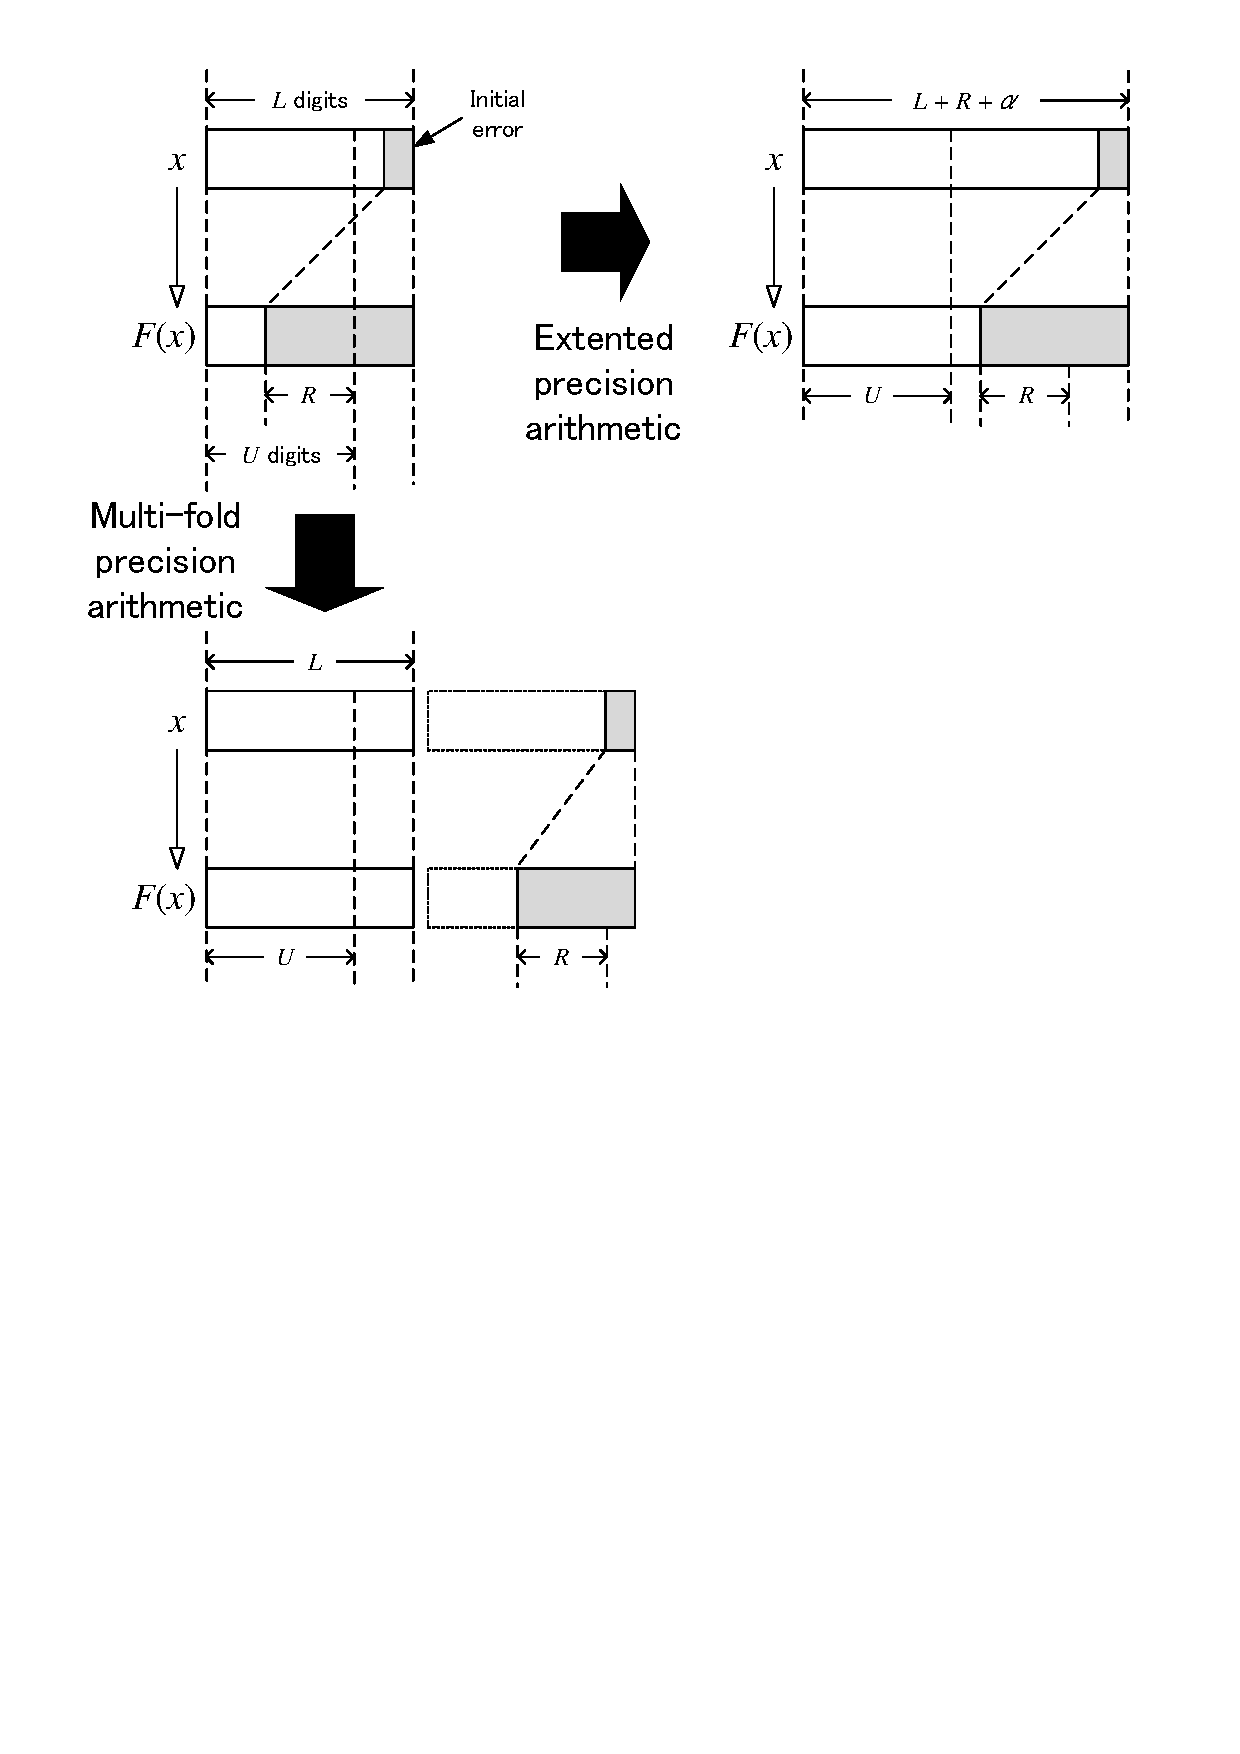
\includegraphics[width=.6\textwidth]{fig/multiprec_multifold.pdf}
        \caption{Extended precision and multi-fold precision arithmetics}
        \label{fig:multiprec_multifold}
    \end{center}
\end{figure}

\bi{Currently, not all algorithms used in numerical computation can be applied using multi-fold arithmetic, especially with nonlinear calculations. Therefore, it is necessary to employ a combination of multi-fold and multiple-precision calculations, where the basic linear calculation part, such as explicit extrapolation process solving initial value problems of ordinary differential equations, uses multi-fold calculations to reduce computational time.}{現在のところ、数値計算で用いられるすべてのアルゴリズム、特に非線形計算をmulti-fold演算で適用できるわけではありません。したがって、multi-foldと多倍長精度計算を組み合わせて用いる必要があり、常微分方程式の初期値問題を解く陽的補外法のような基本線形計算部分にmulti-fold計算を用いることで計算時間を削減します。}

\bi{The Ozaki scheme, a matrix multiplication algorithm that we incorporated into our library, is a technique based on the multi-fold calculation approach. By leveraging the speed of existing binary32 and binary64 xGEMM algorithms, it significantly optimizes multiple-precision matrix multiplication under certain conditions, as revealed in our benchmark and previous studies\cite{mukunoki_binary128}\cite{utsugiri_arxiv2023}. We are confident that the acceleration of multiple-precision linear computation libraries will remain an important theme in guaranteeing the accuracy of broader numerical computation algorithms, following the development trend of multiple-precision numerical algorithms.}{私たちがライブラリに組み込んだ行列乗算アルゴリズムであるOzaki schemeは、multi-fold計算アプローチに基づく技術です。既存のbinary32およびbinary64のxGEMMアルゴリズムの速度を活用することで、私たちのベンチマークおよび先行研究 \cite{mukunoki_binary128}\cite{utsugiri_arxiv2023} で明らかにされているように、特定の条件下で多倍長精度行列乗算を大幅に最適化します。私たちは、多倍長精度数値アルゴリズムの発展動向に従い、多倍長精度線形計算ライブラリの高速化が、より広範な数値計算アルゴリズムの精度保証において引き続き重要なテーマであり続けると確信しています。}

% ---------------------------------------
\section{\bi{Algorithms and performance of optimized matrix multiplication}{最適化された行列乗算のアルゴリズムと性能}}
% ---------------------------------------
\bi{We focused on the optimization of multiple-precision matrix multiplication, starting with MPI support for arbitrary-precision numerical calculations\cite{bnc}. Subsequently, owing to current popularity of multi-core CPUs, we accelerated multiple-precision matrix multiplication via parallelization support using OpenMP. As far as multiple-precision calculations are concerned, no other such results have been achieved by incorporating divide-and-conquer methods, such as the Strassen and Winograd algorithms. Although limited to multi-component methods, our proposed method is the only approach that supports AVX2 and has been converted to OpenMP for achieving higher speeds. However, the current code does not improve performance beyond eight threads for OpenMP acceleration, and a drastic reformulation is necessary to further improve parallelization performance. Algorithm\ \ref{algo:strassen} is the Strassen matrix multiplication.}{私たちは、任意精度数値計算のためのMPIサポート \cite{bnc} を皮切りに、多倍長精度行列乗算の最適化に注力してきました。その後、現在のマルチコアCPUの普及を背景に、OpenMPを用いた並列化サポートによって多倍長精度行列乗算を高速化しました。多倍長精度計算に関する限り、StrassenやWinogradアルゴリズムのような分割統治法を組み込んだ他の同様の成果は得られていません。multi-component方式に限られるものの、私たちの提案手法はAVX2をサポートし、高速化のためにOpenMP化された唯一のアプローチです。しかしながら、現在のコードはOpenMP高速化において8スレッドを超えると性能が向上せず、並列化性能をさらに改善するには抜本的な再構成が必要です。Algorithm\ \ref{algo:strassen} はStrassen行列乗算です。}

%\begin{figure}[htb]
\begin{algorithm}[htb]
    \algsetup{linenosize=\small}
    \small
    \caption{Strassen algorithm for matrix multiplication}\label{algo:strassen}
    \hspace*{\algorithmicindent} \textbf{Input:} $A = [A_{ij}]_{i,j=1,2}\in\mathbb{R}^{m\times l}$, $A_{ij}\in\mathbb{R}^{m/2\times l/2}$, $B = [A_{ij}]_{i,j=1,2}\in\mathbb{R}^{l\times n}$, $B_{ij}\in\mathbb{R}^{l/2\times n/2}$ \\
    \hspace*{\algorithmicindent} \textbf{Output:} $C := \mbox{Strassen}(A, B) = AB\in \mathbb{R}^{m\times n}$
    \begin{algorithmic}
        \IF{$m < m_0$ \&\& $n < n_0$}
            \STATE $C := AB$
        \ENDIF
        \STATE $P_1 := \mbox{Strassen}(A_{11} + A_{22}, B_{11} + B_{22})$
        \STATE $P_2 := \mbox{Strassen}(A_{21} + A_{22}, B_{11})$
        \STATE $P_3 := \mbox{Strassen}(A_{11}, B_{12} - B_{22})$
        \STATE $P_4 := \mbox{Strassen}(A_{22}, B_{21} - B_{11})$
        \STATE $P_5 := \mbox{Strassen}(A_{11} + A_{12}, B_{22})$
        \STATE $P_6 := \mbox{Strassen}(A_{21} - A_{11}, B_{11} + B_{12})$
        \STATE $P_7 := \mbox{Strassen}(A_{12} - A_{22}, B_{21} + B_{22})$
        \STATE $C_{11} := P_1 + P_4 - P_5 + P_7$; $C_{12} := P_3 + P_5$
        \STATE $C_{21} := P_2 + P_4$; $C_{22} := P_1 + P_3 - P_2 + P_6$
        \STATE $C := [C_{ij}]_{i,j=1,2}$
    \end{algorithmic}
\end{algorithm}
%\end{figure}

\bi{The usefulness of the Ozaki scheme is also clear at multiple-precision levels owing to the success of Mukunoki et al. in accelerating the float128 precision matrix multiplication\cite{mukunoki_binary128}.}{Ozaki schemeの有用性は、Mukunokiらによるfloat128精度行列乗算の高速化の成功 \cite{mukunoki_binary128} により、多倍長精度レベルにおいても明らかです。} %The float128 arithmetic, which is supported by GCC, exhibits TD to QD precision performance for addition and multiplication, and is expected to be appropriate for achieving precision levels within this range.
\bi{The float128 arithmetic supported by GCC features TD to QD precision performance for addition and multiplication and is likewise expected to be sufficient for this precision range.}{GCCがサポートするfloat128演算は、加算と乗算においてTDからQD精度の性能を備えており、同様にこの精度範囲に対して十分であると期待されます。}

\bi{The Ozaki scheme is an algorithm that aims to simultaneously accelerate performance and improve accuracy by dividing matrices into more matrices with elements represented by shorter digits. Similarly to the ``Split'' method used in the error-free transformation technique, this approach leverages on the speed of optimized short-precision matrix multiplication (xGEMM) functions. For a given matrix $A \in \mathbb{R}^{m\times l}$ and $B \in \mathbb{R}^{l\times n}$, to obtain a matrix product $C := AB \in \mathbb{R}^{m\times n}$ of long $L$-bit precision, $A$ and $B$ are divided using the Ozaki scheme, where $D \in \mathbb{N}$ is the maximum number of divisions of short $S$-bit precision matrices ($S << L$), as depicted in Algorithm\ \ref{algo:ozaki_scheme}. The $S$-bit arithmetic is used for calculations where no particular description is given, and the $L$-bit arithmetic is used only where high-precision operations are required.}{Ozaki schemeは、行列を、より短い桁で表現される要素を持つ多数の行列に分割することで、性能の高速化と精度の向上を同時に達成することを目指すアルゴリズムです。誤差なし変換技術で用いられる ``Split'' 法と同様に、このアプローチは最適化された短精度行列乗算 (xGEMM) 関数の速度を活用します。与えられた行列 $A \in \mathbb{R}^{m\times l}$ および $B \in \mathbb{R}^{l\times n}$ に対して、長い $L$ ビット精度の行列積 $C := AB \in \mathbb{R}^{m\times n}$ を得るために、Algorithm\ \ref{algo:ozaki_scheme} に示すように、$D \in \mathbb{N}$ を短い $S$ ビット精度行列 ($S << L$) の最大分割数として、$A$ と $B$ はOzaki schemeを用いて分割されます。特に記述のない計算には $S$ ビット演算が用いられ、$L$ ビット演算は高精度演算が必要な箇所でのみ用いられます。}

%\begin{figure}[htb]
\begin{algorithm}[htb]
    \algsetup{linenosize=\small}
    \small
    \caption{Ozaki scheme for multiple-precision matrix multiplication}\label{algo:ozaki_scheme}
	\hspace*{\algorithmicindent} \textbf{Input:} $A \in \mathbb{F}_{bL}^{m\times l}, B \in\mathbb{F}_{bL}^{l\times n}$ \\
	\hspace*{\algorithmicindent} \textbf{Output:} $C \in \mathbb{F}_{bL}^{m\times n}$
    \begin{algorithmic}
        \STATE $A^{(S)} := A$, $B^{(S)} := B$ : $A^{(S)} \in \mathbb{F}_{bS}^{m\times l}$, $B^{(S)} \in \mathbb{F}_{bS}^{l\times n}$
		% divide A and B
		\STATE $\mathbf{e} := [1\ 1\ ...\ 1]^T\in \mathbb{F}_{bS}^l$
		\STATE $\alpha := 1$
		\WHILE{$\alpha < D$}
			\STATE ${\boldsymbol\mu}_A := [\max_{1 \leq p \leq l} |(A^{(S)})_{ip}|]_{i=1, 2, ..., m} \in \mathbb{F}_{bS}^m$
			\STATE ${\boldsymbol\mu}_B := [\max_{1 \leq q \leq l} |(B^{(S)})_{qj}|]_{j=1, 2, ..., n} \in \mathbb{F}_{bS}^n$
			\STATE ${\boldsymbol\tau}_A := [2^{\lceil \log_2(({\boldsymbol\mu}_A)_i)\rceil + \lceil (S + \log_2(l)) / 2 \rceil} ]_{i = 1, 2, ..., m} \in \mathbb{F}_{bS}^m$
			\STATE ${\boldsymbol\tau}_B := [2^{\lceil \log_2(({\boldsymbol\mu}_B)_j)\rceil + \lceil (S + \log_2(l)) / 2 \rceil} ]_{j = 1, 2, ..., n} \in \mathbb{F}_{bS}^n$
			\STATE $S_A := \boldsymbol\tau_A \mathbf{e}^T$
			\STATE $S_B := \mathbf{e} \boldsymbol\tau_B^T$
			\STATE $A_\alpha := (A^{(S)} + S_A) - S_A$: $A_\alpha \in \mathbb{F}_{bS}^{m\times l}$
			\STATE $B_\alpha := (B^{(S)} + S_B) - S_B$: $B_\alpha \in \mathbb{F}_{bS}^{l\times n}$
			\STATE $A := A - A_\alpha$, $B := B - B_\alpha$ : $L$-bit FP arithmetic
			\STATE $A^{(S)} := A$, $B^{(S)} := B$
			\STATE $\alpha := \alpha + 1$  
		\ENDWHILE
		% multiplication
		\STATE $A_D := A^{(S)}$, $B_D := B^{(S)}$
		\STATE $C := O$
		\FOR{$\alpha = 1, 2, ..., D$}
			\FOR{$\beta = 1, 2, ..., D - \alpha + 1$}
				\STATE $C_{\alpha\beta} := A_\alpha B_\beta$
			\ENDFOR
			\STATE $C := C + \sum^{D - \alpha + 1}_{\beta = 1} C_{\alpha\beta}$ : $L$-bit FP arithmetic
		\ENDFOR
    \end{algorithmic}
\end{algorithm}
%\end{figure}

\bi{\figurename\ref{fig:ozaki_scheme3x3} illustrates an example of the Ozaki scheme when $A$ and $B\in\mathbb{R}^{3\times 3}$ are divided into three short-digit matrices.}{\figurename\ref{fig:ozaki_scheme3x3} は、$A$ と $B\in\mathbb{R}^{3\times 3}$ を3つの短桁行列に分割した場合のOzaki schemeの例を示しています。}
\begin{figure}[htb]
	\begin{center}
		%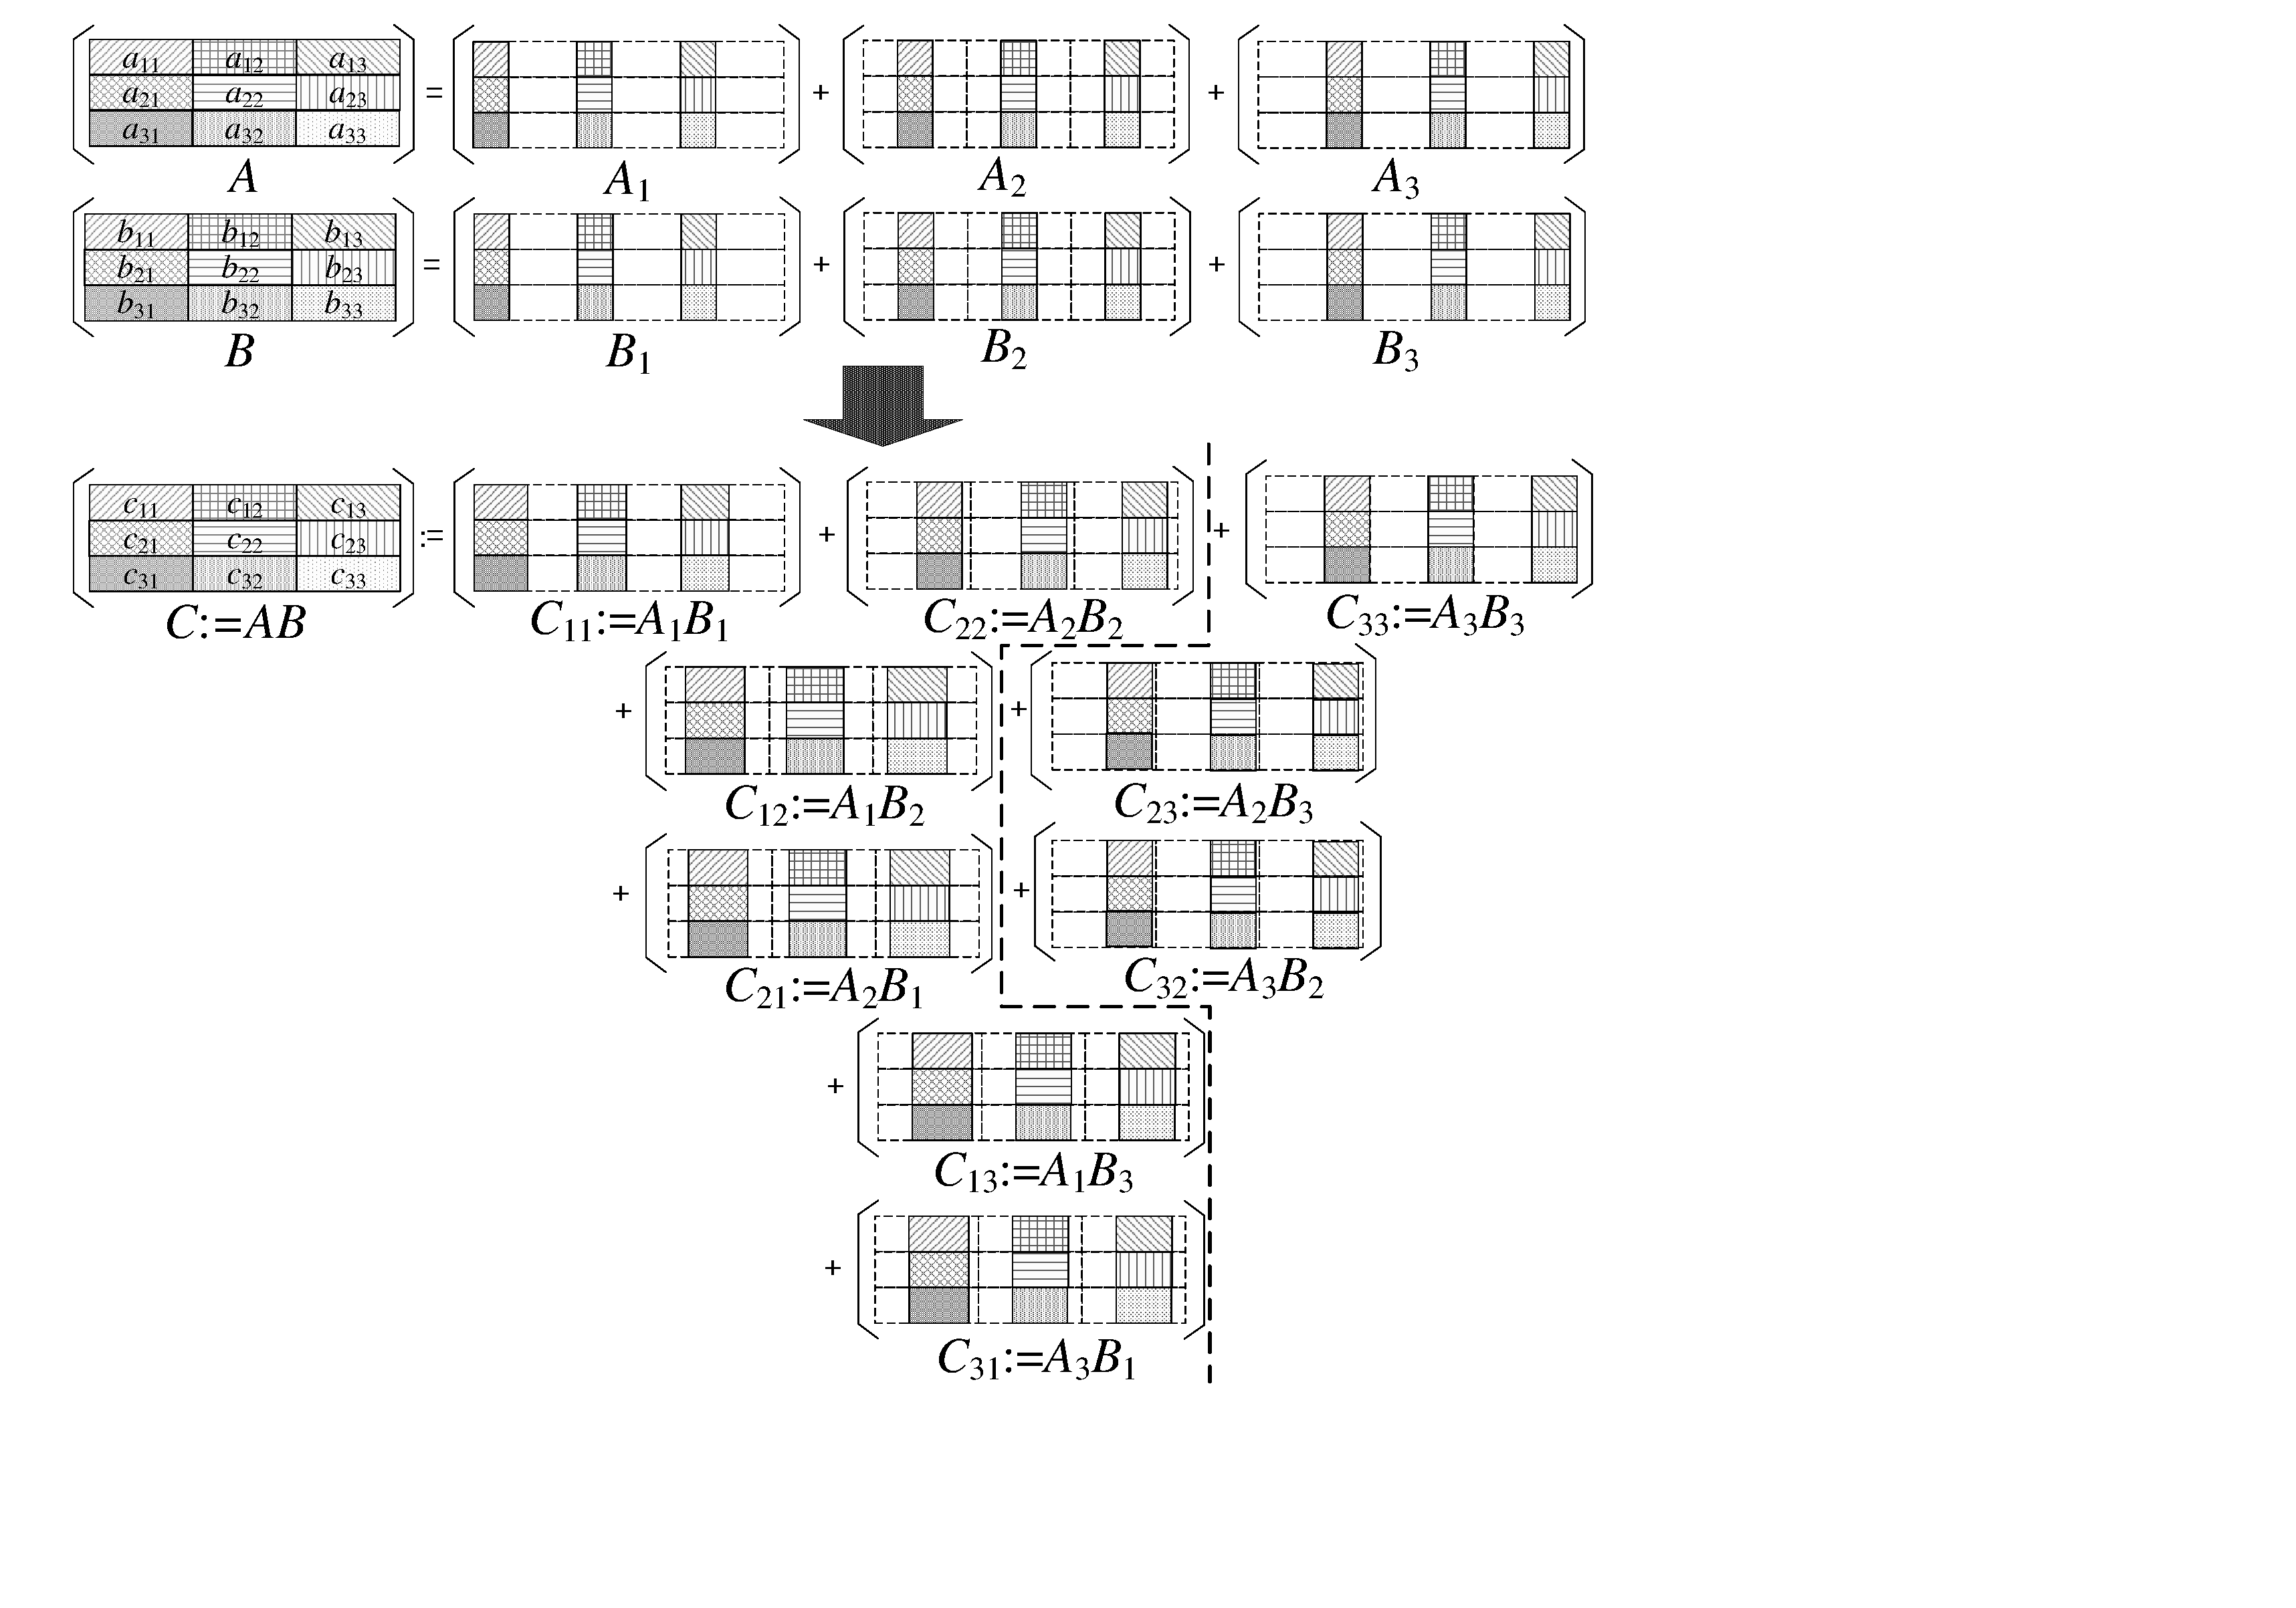
\includegraphics[width=.75\textwidth]{fig/ozaki_scheme_3x3.pdf}
		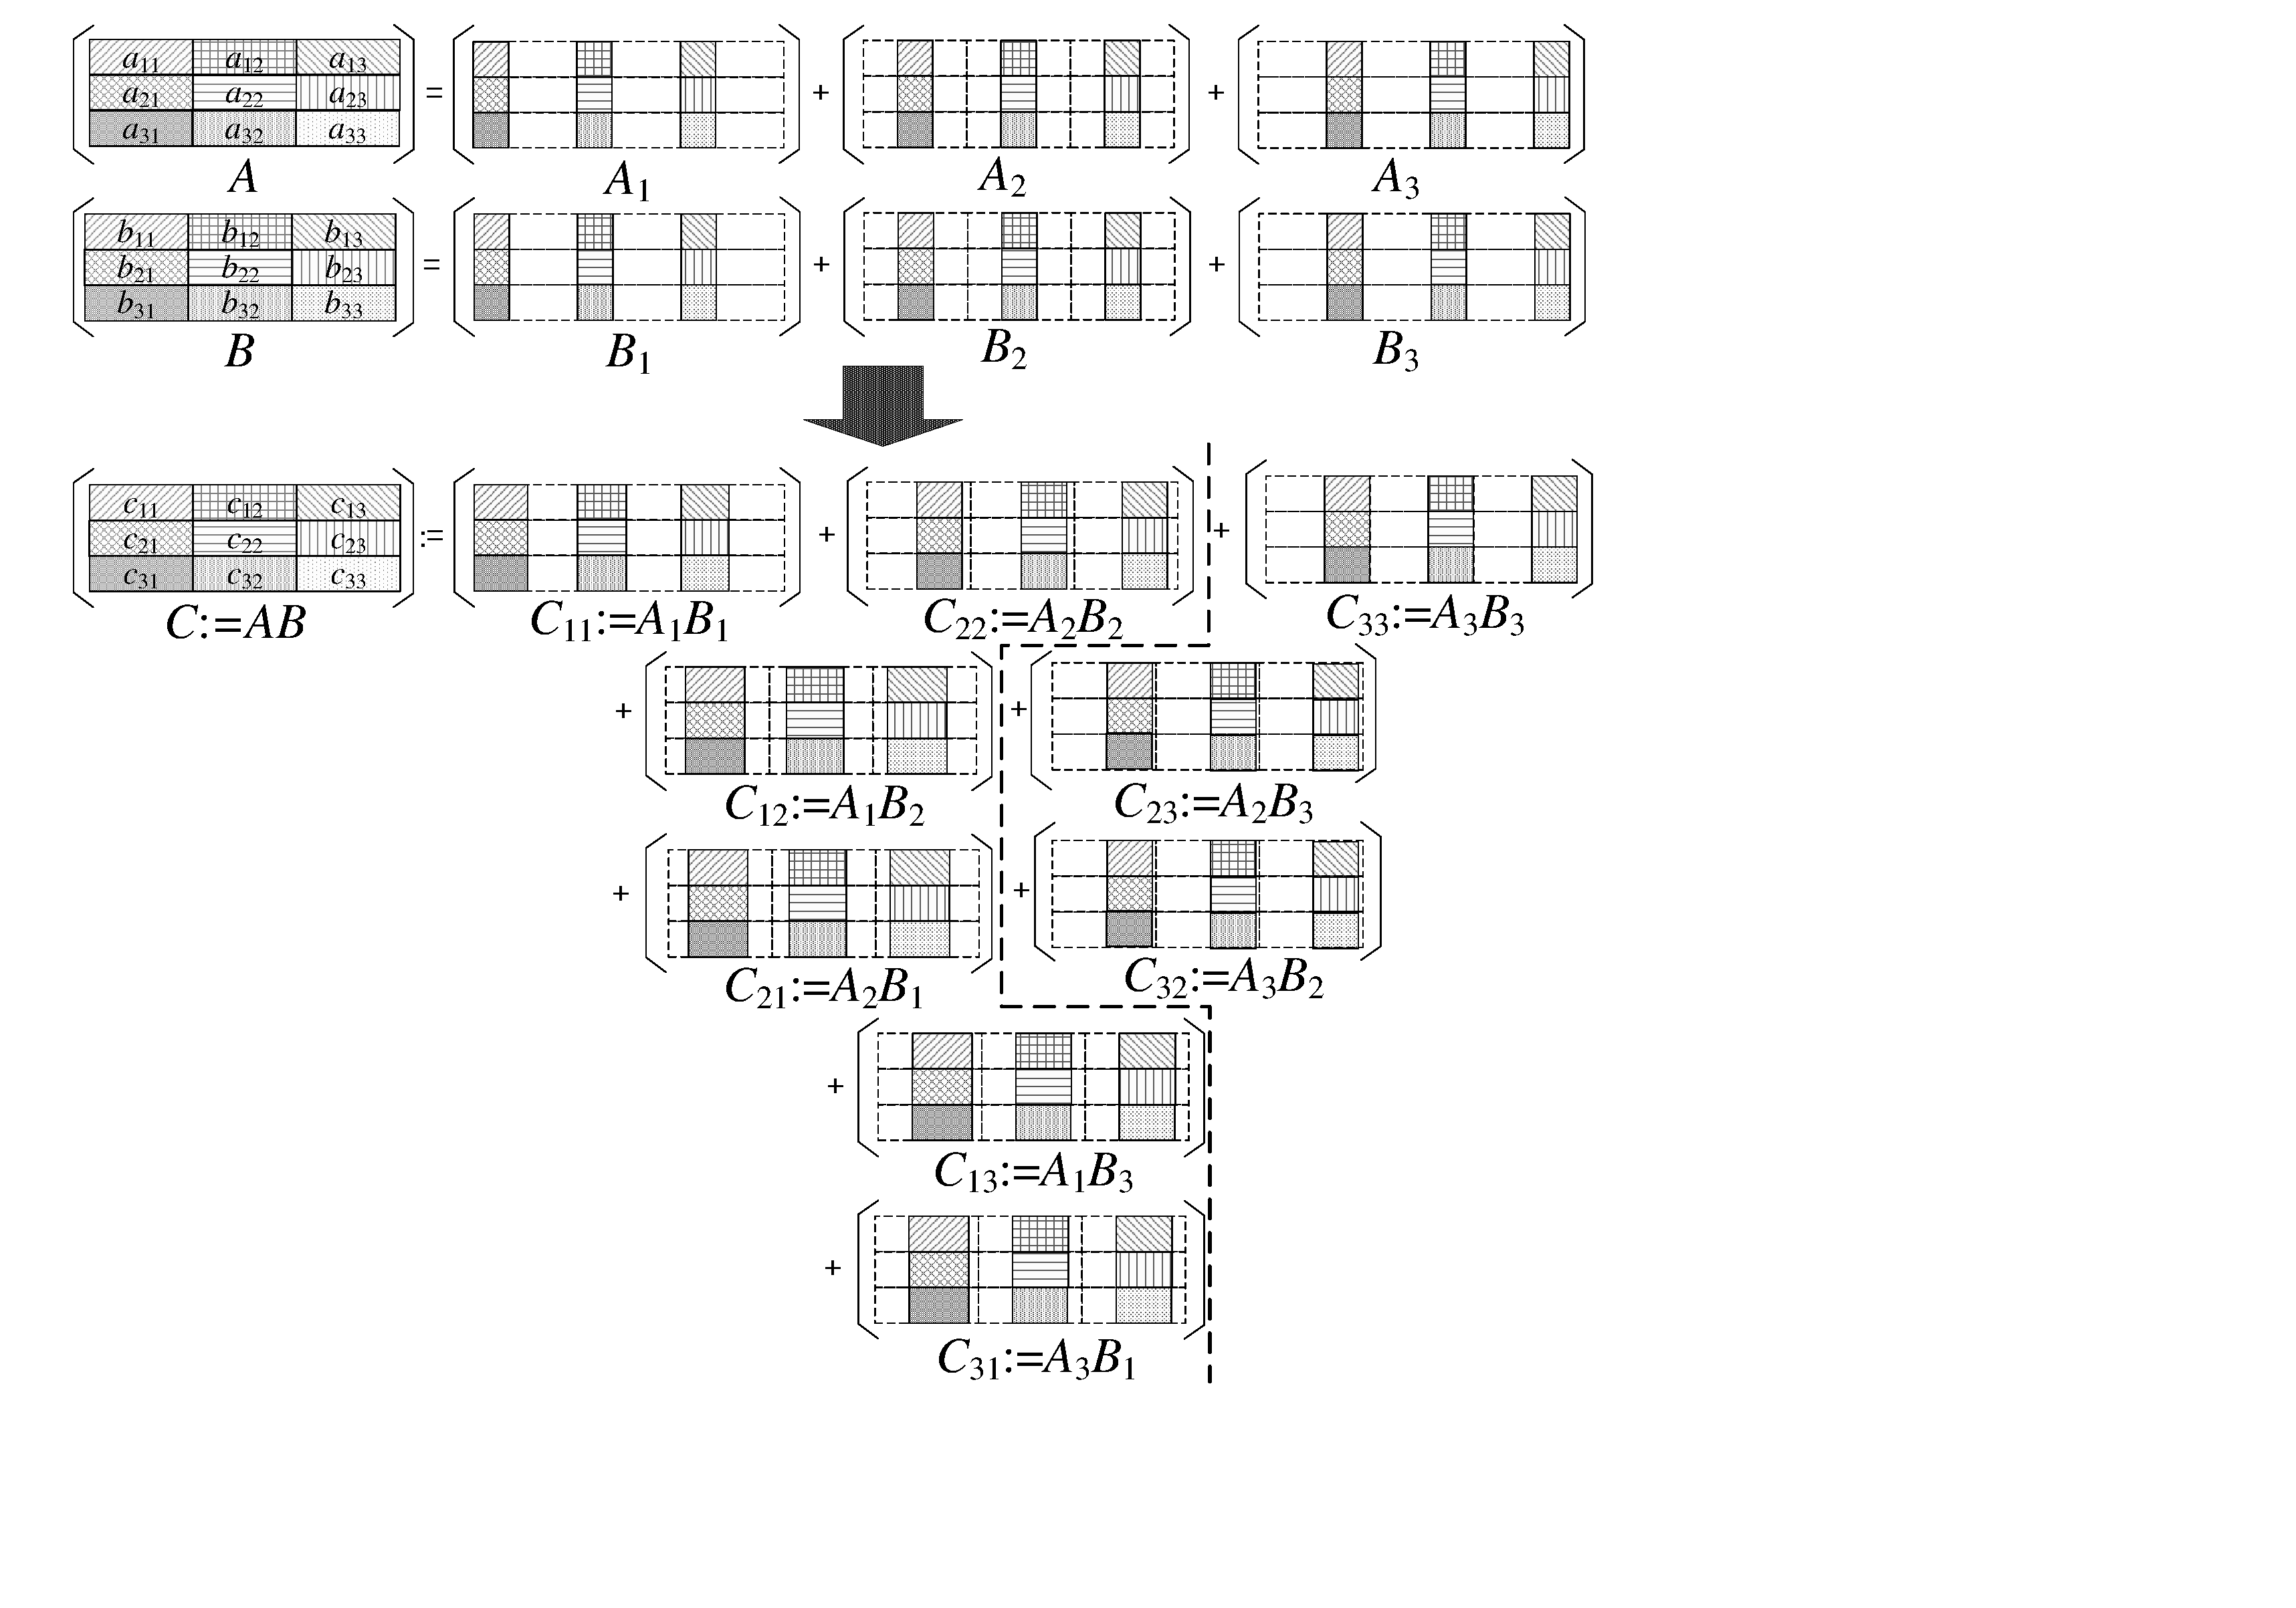
\includegraphics[width=.7\textwidth]{fig/ozaki_scheme_3x3.pdf}
        \caption{Matrix multiplication based on Ozaki scheme when the matrices are divided into three components}
		\label{fig:ozaki_scheme3x3}
	\end{center}
\end{figure}
\bi{The most important feature of the Ozaki scheme is that the matrices $A$ and $B$ are divided into $A_1$, $A_2$, $A_3$, $B_1$, $B_2$, and $B_3$ to fit within a short precision, thereby avoiding rounding errors in fast, low-precision matrix multiplication. An error-free matrix product $C_{ij} := A_i B_j$$(i,j=1, 2, 3)$ can be obtained as a result, and a highly accurate matrix product $C$ can be obtained using a multiple-precision matrix addition operation for $C := \sum_{i,j} C_{ij}$. Although the number of divisions of $A$ and $B$ is finite, it is difficult to determine the minimum number of divisions required to guarantee a certain accuracy threshold. As a result, benchmark tests must be performed to determine if the algorithm can be executed faster than other multiplication algorithms.}{Ozaki schemeの最も重要な特徴は、行列 $A$ と $B$ が短精度に収まるように $A_1$、$A_2$、$A_3$、$B_1$、$B_2$、$B_3$ に分割され、それによって高速な低精度行列乗算における丸め誤差を回避できる点です。その結果として誤差なし行列積 $C_{ij} := A_i B_j$$(i,j=1, 2, 3)$ を得ることができ、$C := \sum_{i,j} C_{ij}$ という多倍長精度行列加算演算を用いて高精度な行列積 $C$ を得ることができます。$A$ と $B$ の分割数は有限ですが、ある精度のしきい値を保証するために必要な最小分割数を決定することは困難です。その結果、このアルゴリズムが他の乗算アルゴリズムよりも高速に実行できるかどうかを判断するには、ベンチマークテストを行う必要があります。}

% ---------------------------------------
\section{\bi{Software layer of BNCmatmul}{BNCmatmulのソフトウェア層}}
% ---------------------------------------

\bi{We have already used QD\cite{qd} as multi-component-type fixed precision C++ class library, CAMPARY\cite{campary_paper2016} as multi-component-type arbitrary precision library, and MPFR\cite{mpfr} baased on GNU MP\cite{gmp}'s MPN kernel. MPLAPACK/MPBLAS\cite{mplapack} is greeding these all reliable MP libraries and providing the coresponding APIs of LAPACK/BLAS\cite{lapack}.}{私たちはこれまで、multi-component型固定精度C++クラスライブラリとしてQD \cite{qd}、multi-component型任意精度ライブラリとしてCAMPARY \cite{campary_paper2016}、そしてGNU MP \cite{gmp} のMPNカーネルに基づくMPFR \cite{mpfr} を用いてきました。MPLAPACK/MPBLAS \cite{mplapack} は、これらすべての信頼できる多倍長精度ライブラリを取り込み、LAPACK/BLAS \cite{lapack} に対応するAPIを提供しています。}
\bi{Our BNCmatmul developed aims to get better performance than MPBLAS as ATLAS, OpenBLAS and Intel Math Kernel, and it has the following features:}{私たちが開発したBNCmatmulは、ATLAS、OpenBLAS、Intel Math KernelのようにMPBLASよりも優れた性能を得ることを目指しており、以下の特徴を持ちます。}
\begin{itemize}
    \item \bi{Core functions and macros are wriiten in the traditional way of ANSI C, not C++.}{中核となる関数とマクロは、C++ではなく従来のANSI Cの流儀で書かれています。}
    \item \bi{Supporting native multi-component-type DD, TD, and QD precision arithmetic, and also accelelating vector and matrix computation like BLAS with AVX2 and AVX-512 on x86-64, and NEON and SVE2 on AArch64. As of 0.24 the AVX-512 backend covers every kernel the AVX2 backend does and is verified bit-identical to the scalar one (Sec.~\ref{sec:simdbackends}).}{ネイティブなmulti-component型のDD、TD、QD精度演算をサポートし、さらにx86-64ではAVX2とAVX-512、AArch64ではNEONとSVE2を用いてBLASのようにベクトルおよび行列計算を高速化します。0.24の時点でAVX-512バックエンドはAVX2バックエンドと同一のカーネルをすべて備え、スカラー版とのビット一致が検証されています（\ref{sec:simdbackends}節）。}
    \item \bi{Direct use of MPFR functions to avoid overhead due to mpreal class library.}{mprealクラスライブラリによるオーバーヘッドを回避するために、MPFR関数を直接利用します。}
    \item \bi{Supporting partly shared-memory-type parallelization based on OpenMP.}{OpenMPに基づく共有メモリ型並列化を部分的にサポートします。}
    \item \bi{Implementing three algorightms of matrix multiplication: simple triple-loop, blocking (tiling), and Strassen or Winograd algorithm. Ozaki scheme can be used as trial optimization.}{行列乗算の3つのアルゴリズム、すなわち単純な三重ループ、ブロック化 (タイリング)、およびStrassenまたはWinogradアルゴリズムを実装しています。Ozaki schemeは試験的な最適化として利用できます。}
\end{itemize}

\bi{The software layer of BNCmatmul except parallelization is shown as \figurename\ref{fig:lu_bench_layer}.}{並列化を除いたBNCmatmulのソフトウェア層を \figurename\ref{fig:lu_bench_layer} に示します。}

\begin{figure}[htb]
    \begin{center}
        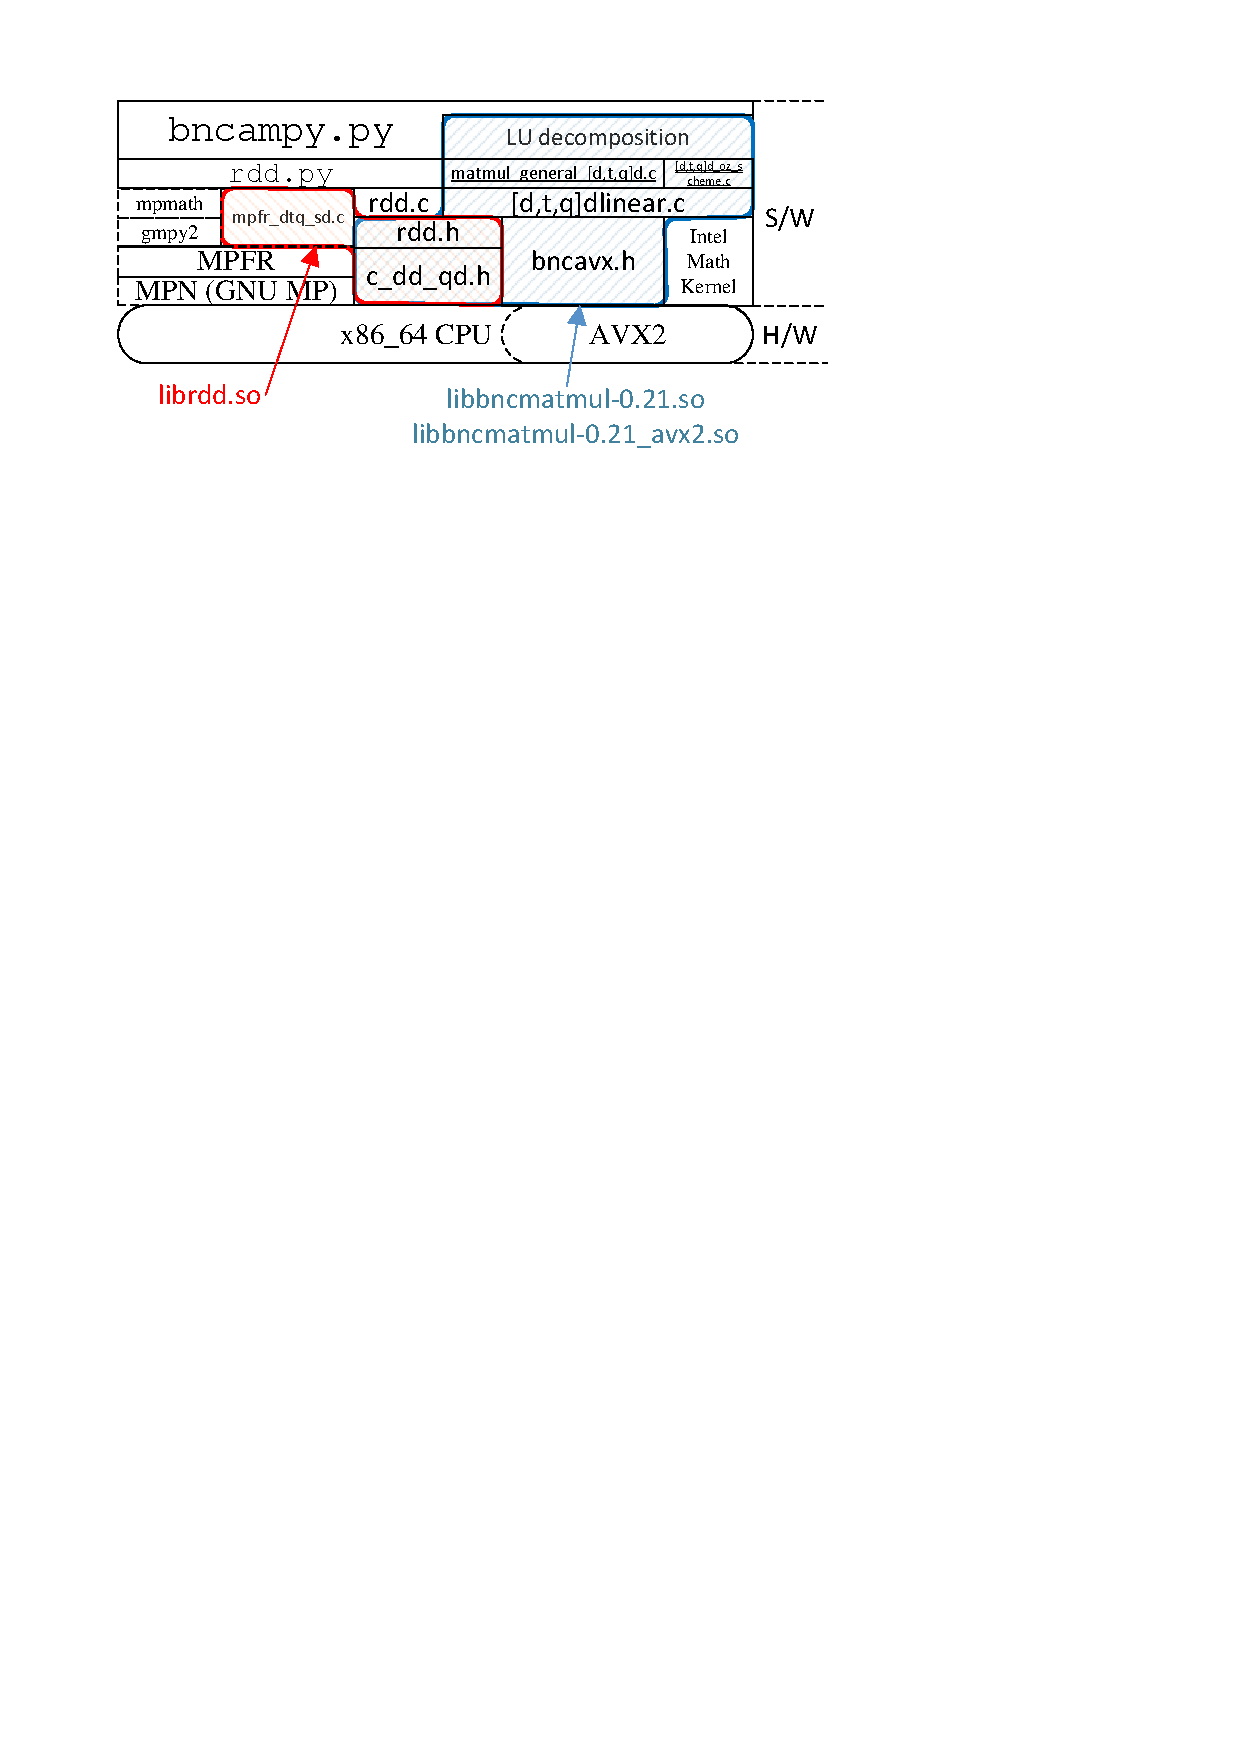
\includegraphics[width=.45\textwidth]{fig/pyrdd.pdf}
        \caption{Software layer of BNCmatmul library}
        \label{fig:lu_bench_layer}
    \end{center}
\end{figure}


\bi{Basic DD, TD, and QD precision arithmetic are defined as C inline functions in c\_dd\_qd.h and are defined as macros in rdd.h. To use the Python environment, rdd.c, which is based on rdd.h, is compiled as librdd.so. The DD, TD, and QD classes on Python use the functions defined in librdd.so.}{基本的なDD、TD、QD精度演算は、c\_dd\_qd.h内でCのinline関数として定義され、rdd.h内でマクロとして定義されています。Python環境を利用するために、rdd.hに基づくrdd.cがlibrdd.soとしてコンパイルされます。Python上のDD、TD、QDクラスは、librdd.so内で定義された関数を用います。}

\bi{BNCmatmul, which is also built on rdd.h and c\_dd\_qd.h, includes block and Strassen matrix multiplications that provide more efficient performance than simple triple-loop matrix multiplication. These have been accelerated using the SIMDized functions defined under include/avx2/ --- \texttt{\_bncavx\_*.h} for AVX2 (\texttt{\_\_m256d}/\texttt{\_\_m256}) and \texttt{\_bncavx\_*\_avx512.h} for AVX-512 (\texttt{\_\_m512d}/\texttt{\_\_m512}), both reached through the umbrella header avx2/bncavx.h --- and by their counterparts under include/neon/ and include/sve2/ on AArch64. The LU decomposition has also been accelerated in the same way.}{同じくrdd.hおよびc\_dd\_qd.h上に構築されたBNCmatmulには、単純な三重ループ行列乗算よりも効率的な性能を提供するブロック行列乗算およびStrassen行列乗算が含まれています。これらは、include/avx2/以下で定義されたSIMD化関数 --- AVX2用の \texttt{\_bncavx\_*.h}（\texttt{\_\_m256d}/\texttt{\_\_m256}）とAVX-512用の \texttt{\_bncavx\_*\_avx512.h}（\texttt{\_\_m512d}/\texttt{\_\_m512}）で、いずれもアンブレラヘッダ avx2/bncavx.h 経由で取り込まれます --- および、AArch64ではinclude/neon/・include/sve2/以下の対応する関数を用いて高速化されています。LU分解も同様に高速化されています。}

\bi{These functions that are defined in BNCmatmul (\figurename\ \ref{fig:lu_bench_layer}) can be used from libbncmatmul-0.xx.a/.so without any SIMDization techniques, and from libbncmatmul-0.xx\_avx2, \_avx512, \_neon, and \_sve2 with the SIMDization of AVX2, AVX-512, Arm NEON and Armv9-A SVE2, respectively. As these libraries have the same function names, so users do not need to modify their codes when selecting the BNCmatmul library --- the SIMD backend is chosen at link time only.}{BNCmatmul (\figurename\ \ref{fig:lu_bench_layer}) で定義されたこれらの関数は、SIMD化技術を用いないlibbncmatmul-0.xx.a/.so、およびAVX2・AVX-512・Arm NEON・Armv9-A SVE2によるSIMD化をそれぞれ用いたlibbncmatmul-0.xx\_avx2・\_avx512・\_neon・\_sve2から利用できます。これらのライブラリは同じ関数名を持つため、ユーザはBNCmatmulのライブラリを選択する際にコードを変更する必要はありません。SIMDバックエンドはリンク時にのみ選択されます。}


%------------------------------------------------%
% Todo list
%------------------------------------------------%
\section{\bi{History of Version and Todo list}{バージョン履歴とTodoリスト}}

\paragraph{\bi{History of Version}{バージョン履歴}}

\begin{description}
    \item[Version 0.24: 2026-08-15] \bi{Certified branch-free FMA and FMA-based elementary functions, ported from dtq-0.0.3 in plain ANSI C:}{dtq-0.0.3から純粋なANSI Cで移植した、証明付きbranch-free FMAとFMAベース初等関数:}
    \begin{enumerate}
        \item \bi{Branch-free fused multiply-add kernels \texttt{bnc\_\{dw,tw,qw\}fma[f]} with machine-proved error bounds (\texttt{bncfma.h}), including SIMD versions for NEON, SVE2, and --- newly --- AVX2/AVX-512 (\texttt{avx2/\_bncavx\_fma.h}); the NEON and AVX2 kernels are verified bit-identical to the scalar certified ones (Sec.~\ref{sec:bncfma})}{機械証明された誤差限界を持つbranch-free融合積和カーネル \texttt{bnc\_\{dw,tw,qw\}fma[f]}（\texttt{bncfma.h}）。NEON・SVE2に加え、新たにAVX2/AVX-512版（\texttt{avx2/\_bncavx\_fma.h}）を追加。NEON版・AVX2版はスカラー認証版とのビット一致を検証済み（\ref{sec:bncfma}節）}
        \item \bi{FMA-fused elementary functions $\exp$, $\mathrm{expm1}$, $\log$, $\log_{10}$, $\sin$, $\cos$, $\mathrm{sincos}$ for DD/TD/QD (DS/TS/QS by delegation), replacing the previous empty stubs and missing implementations of \texttt{c\_dd\_sin}, \texttt{c\_td\_*}, \texttt{c\_qd\_*}, etc.; accuracy validated against MPFR, average error below $1\,\varepsilon$ of each type (Sec.~\ref{sec:bncelem})}{DD/TD/QD向けFMA融合初等関数 $\exp$・$\mathrm{expm1}$・$\log$・$\log_{10}$・$\sin$・$\cos$・$\mathrm{sincos}$（DS/TS/QSは委譲）。従来の \texttt{c\_dd\_sin}・\texttt{c\_td\_*}・\texttt{c\_qd\_*} 等の空スタブ・未実装を置き換え。MPFR基準で精度検証済み、平均誤差は各型の$1\,\varepsilon$未満（\ref{sec:bncelem}節）}
        \item \bi{Elementwise array functions \texttt{bnc\_\{dd,td,qd\}\_\{exp,log,sin,cos\}\_array} over limb-planar arrays, blocked by the SIMD width of the build and bitwise identical to the scalar functions (Sec.~\ref{sec:bncelem})}{limb-planar配列に対する一括関数 \texttt{bnc\_\{dd,td,qd\}\_\{exp,log,sin,cos\}\_array}。ビルドのSIMD幅でブロック化され、スカラー関数とビット単位で一致（\ref{sec:bncelem}節）}
        \item \bi{Bug fixes: \texttt{const\_dd\_pi} held $\pi/16$, \texttt{const\_td\_pi}/\texttt{const\_qd\_pi} held $\pi/1024$, single-based $\pi$ constants were zero, and \texttt{c\_dd\_nint} was an empty stub}{バグ修正: \texttt{const\_dd\_pi} が$\pi/16$、\texttt{const\_td\_pi}/\texttt{const\_qd\_pi} が$\pi/1024$、float基の$\pi$定数がゼロ、\texttt{c\_dd\_nint} が空スタブだった問題}
        \item \bi{div/sqrt-safe FMA variants \texttt{bnc\_\{dw,tw,qw\}fma[f]\_safe} and the FMA-driven divisions \texttt{bnc\_\{dd,td,qd,ds,ts,qs\}\_div\_fma} (dtq \texttt{fma\_div} ports; opt-in default switch \texttt{BNC\_USE\_FMA\_DIV}); the double-based divisions run $1.2\times$/$2.8\times$/$2.2\times$ (DD/TD/QD) faster at the same accuracy (Sec.~\ref{sec:fmadiv})}{div/sqrt-safe版FMA \texttt{bnc\_\{dw,tw,qw\}fma[f]\_safe} とFMA駆動除算 \texttt{bnc\_\{dd,td,qd,ds,ts,qs\}\_div\_fma}（dtqの\texttt{fma\_div}移植。\texttt{BNC\_USE\_FMA\_DIV} で既定除算を切替可能）。double基の除算は同精度のまま$1.2$倍／$2.8$倍／$2.2$倍（DD/TD/QD）高速（\ref{sec:fmadiv}節）}
        \item \bi{AVX-512 backend brought to parity with AVX2: 411 of the 426 AVX2 constructs in the compiled sources now have a matching AVX-512 arm, the \texttt{avx512} build needs no ISA beyond AVX-512F + FMA, and the serial, AVX2 and AVX-512 builds are verified bit-identical on the element-wise and sparse kernels (Sec.~\ref{sec:simdbackends})}{AVX-512バックエンドをAVX2と同等に整備: ビルド対象ソース中426個のAVX2構文のうち411個が対応するAVX-512の腕を備え、\texttt{avx512} ビルドに必要なISAはAVX-512F + FMAのみ。serial・AVX2・AVX-512の各ビルドが要素毎カーネルおよび疎行列カーネルでビット一致することを検証済み（\ref{sec:simdbackends}節）}
        \item \bi{DLL-ready exported function API \texttt{rdd\_*}/\texttt{rtd\_*}/\texttt{rqd\_*}/\texttt{rds\_*}/\texttt{rts\_*}/\texttt{rqs\_*} (99 symbols, \texttt{src/rdtq\_func.c} + \texttt{include/rdtq\_func.h}) for Python/ctypes, with the \texttt{librdtq} build target and the \texttt{python/test\_rdtq.py} driver (Sec.~\ref{sec:rdtqfunc})}{Python/ctypes向けのDLL対応関数エクスポートAPI \texttt{rdd\_*}/\texttt{rtd\_*}/\texttt{rqd\_*}/\texttt{rds\_*}/\texttt{rts\_*}/\texttt{rqs\_*}（99シンボル、\texttt{src/rdtq\_func.c} + \texttt{include/rdtq\_func.h}）。\texttt{librdtq} ビルドターゲットと \texttt{python/test\_rdtq.py} ドライバ付き（\ref{sec:rdtqfunc}節）}
    \end{enumerate}
    \item[Version 0.23: 2026-03-16] \bi{BNCmatmul accelerated on Arm Neon CPUs has been released.}{Arm Neon CPU上で高速化されたBNCmatmulがリリースされました。}
    \item[Version 0.22: 2024-05-31] \bi{Some functions have been appended:}{いくつかの関数が追加されました。}
    \begin{enumerate}
        \item \bi{Complex arithmetic and linear computation}{複素数演算と線形計算}
        \item \bi{Miscellaneous functions (accessares, elementary and random functions) }{各種関数 (アクセサ、初等関数、乱数関数)}
        \item \bi{Sparse matrix and SpMV}{疎行列とSpMV}
    \end{enumerate}
    \item[Version 0.21: 2023-05-31] \bi{Secondly opening sources including DD, TD, QD and MPFR precision real BLAS functions at \url{https://github.com/tkouya/bncmatmul/blob/main/bncmatmul-0.21.tar.bz2}.}{DD、TD、QD、MPFR精度の実数BLAS関数を含むソースを \url{https://github.com/tkouya/bncmatmul/blob/main/bncmatmul-0.21.tar.bz2} で2回目に公開しました。}
    \item[Version 0.20: 2016-06-08] \bi{Firstly opening sources at \url{https://na-inet.jp/na/bnc/bncmatmul-0.2.tar.bz2}, which provides only artibrary matrix multiplication based on MPFR.}{MPFRに基づく任意精度行列乗算のみを提供するソースを \url{https://na-inet.jp/na/bnc/bncmatmul-0.2.tar.bz2} で初めて公開しました。}
\end{description}

\paragraph{\bi{Todo list}{Todoリスト}}

\begin{enumerate}
    %\item Appending complex BLAS functions with DD, TD, QD, and MPFR(MPC)
    %\item Appending complex LU decomposition and related functions
    %\item Appending sparse matrix-vector multiplication
    \item \bi{Showing more sample sources in this manual using BNCmatmul and MPLAPACK/BLAS}{本マニュアルにおいて、BNCmatmulとMPLAPACK/BLASを用いたサンプルソースをより多く示すこと}
    \item \bi{Completing descriptions of our library usage and how to apply various situations with it.}{本ライブラリの使用方法と、さまざまな状況への適用方法に関する説明を完成させること}
\end{enumerate}

%------------------------------------------------%
% End of Document
%------------------------------------------------%